\documentclass{article}
\usepackage[utf8]{inputenc}
\usepackage{hyperref}
%\usepackage{amsmath}
%\usepackage{amsfonts}
%\usepackage{amssymb}
%\usepackage{amsthm}
\usepackage{mathtools}
\usepackage{graphicx}
\graphicspath{ {./images/} }
\usepackage{pgfplots}
\pgfplotsset{width=10cm,compat=1.9}
\usepackage{amsmath}
\usepackage{setspace}
\usepackage{amsbsy}
\usepackage{amssymb}
\usepackage[utf8]{inputenc}
\usepackage{multirow}
\usepackage[ruled,vlined]{algorithm2e}
\usepackage{algorithmic}
\DeclareUnicodeCharacter{2212}{-}
\usepackage[utf8]{inputenc}
\numberwithin{figure}{section}
\usepackage[]{algorithm2e}
\usepackage{minted}
\usepackage{listings}
\usepackage{caption}
\usepackage{multicol}
\usepackage{setspace}
\usepackage{chngcntr}
\usepackage{array}
\usepackage{verbatim}
\newenvironment{metaverbatim}{\verbatim}{\endverbatim}

\let\oldemptyset\emptyset
\let\emptyset\varnothing

\lstset{
language=C,
basicstyle=\small\ttfamily,
numbers=left,
numbersep=5pt,
xleftmargin=20pt,
frame=tb,
framexleftmargin=20pt
}

\renewcommand*\thelstnumber{\arabic{lstnumber}:}

\DeclareCaptionFormat{mylst}{\hrule#1#2#3}
\captionsetup[lstlisting]{format=mylst,labelfont=bf,singlelinecheck=off,labelsep=space}

\usepackage{pdfrender}
\DeclareRobustCommand*{\pmbb}[1]{%
  \textpdfrender{
    TextRenderingMode=Stroke,
    LineWidth=.1pt,
  }{#1}%
}

\title{A practical and theoretical analysis in the comparison of sorting algorithms}
\author{Șova Dumitru Ștefan Andrei\\
Department of Computer Science, \\
West Univesity, \\
Timișoara, Romania, \\
Email: \href{mailto:dumitru.sova01@e-uvt.ro}{\texttt{dumitru.sova01@e-uvt.ro}}
}
\date{June 2021}

\begin{document}

\maketitle
\begin{abstract}
One of the main points of interest regarding sorting algorithms stems from their respective time complexity. Be it old or new each algorithm has a specific complexity that can create a reference that can be used in a comparison with other such algorithms. Theoretically, the description of the complexity and its analysis, alongside experimental tests conducted at different input values can provide a starting point in contrasting sorting algorithms. In this paper, we compare several sorting algorithms, analyzing them both theoretically and experimentally in regard to their complexity. The algorithms used are Bubble Sort, Insertion Sort, Merge Sort, Quicksort, Heapsort, Radix Sort, and Counting Sort, which were implemented in the C programming language using Codeblocks.


\end{abstract}
\pagebreak
 

\section{Introduction}

Sorting algorithms represent some of the building blocks of Computer Science, acquiring a keen interest in their analysis through large amounts of research. As such, these algorithms are well-established and documented design and performance-wise. With this, the purpose of the paper is to give a better understanding of the time complexity of several well-known sorting algorithms by comparing them with one another.

The data used for the experiments was generated in C, creating lists of randomly sorted integer numbers ranging from 10 000 to 1 million elements. The complexity of each algorithm was analyzed both theoretically, describing their behavior and properties, and practically, experiments being conducted in regards to the run times of the algorithms at said data inputs.

\subsection{Motivation}

The problem of comparing sorting algorithms arises from the multitude of already documented algorithms and the desire to find the most efficient one. We can become, as such, overwhelmed by the amount of currently studied sorting algorithms. For example, when sorting sizeable amounts of data inputs, the difficulty of choosing a preferred algorithm can become an inconvenience, some algorithms(Quicksort, Radix Sort) outperforming others(Bubble sort, Selection sort) by a wide margin when it comes to time efficiency. Such differences can be seen in Figure~\ref{fig:exp1}. As such, we become compelled to think that there exists a definitive best sorting algorithm that is yet to be encountered by us, but the fact of the matter is that a convenient enough algorithm is not so easily identifiable. Because of this, different sorting algorithms might be more desirable over others depending on the data type, how the data is represented, and the input distribution. Another example would be when trying to sort nearly sorted data, Insertion Sort proving to be a good choice for this type of scenario, whilst Quicksort, Merge Sort, and Heap Sort adapting at a slower rate to this type of distribution. With these facts in mind, the problem of comparing sorting algorithms might not have a definitive answer, but it might offer a more detailed look when choosing one.

Roughly the steps for the comparison of the sorting algorithms proceed as follows:
\begin{itemize}
\item The plan for the comparison is to analyze their respective complexity and to compare at different data inputs ranging from 10 000 to 1 million elements the time each algorithm takes to sort a list of elements.
\pagebreak

\item The first step is to implement the sorting algorithms that we will end up comparing, those being Bubble Sort, Insertion Sort, Merge Sort, Quicksort, Heapsort, Radix Sort, and Counting Sort. To do this, we will use the C language and Codeblocks to write the code.

\item The data inputs will be generated in C, creating lists between 10 000 to 1 million elements that will have random integer values.

\item With the data inputs created, each algorithm will run said inputs and offer results that are going to be used in the comparison.

\item The complexity and other properties of each algorithm will be analyzed and will become a base of comparison between the algorithms in regards time.

\item With both the sorting time and complexity analysis done, we can begin the proper comparison and produce results.

\item The expected outcome is that some algorithms will fare better than others, namely Quicksort, Merge Sort, Radix Sort, and Heapsort, especially when looking at large data inputs that exceed 500 000 elements.
\end{itemize}

\begin{figure}[h]
    \centering
    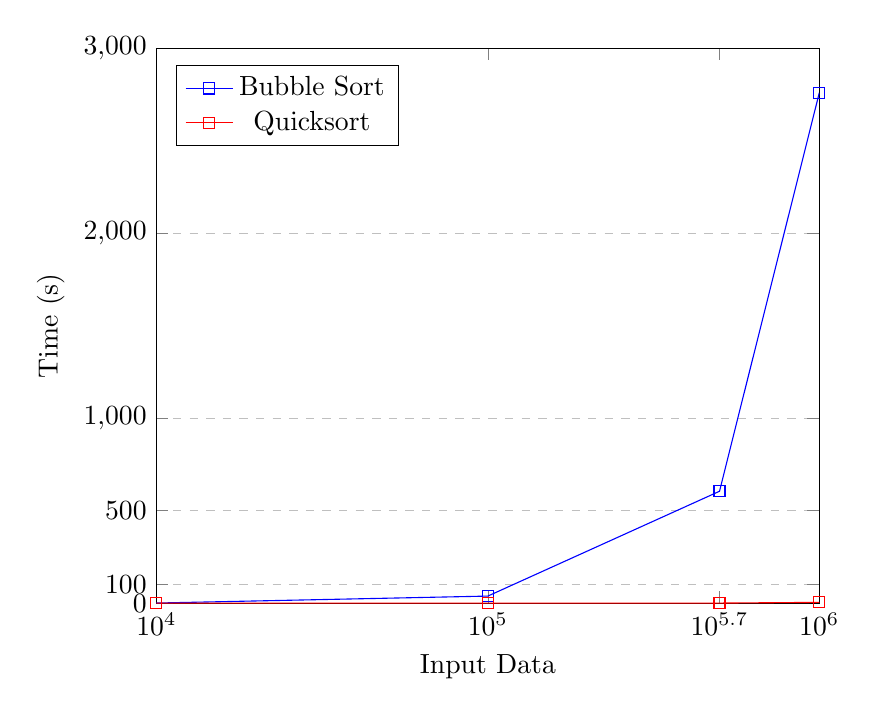
\begin{tikzpicture}
    \begin{semilogxaxis}[
        xlabel={Input Data},
        ylabel={Time (s)},
        xmin=10000, xmax=1000000,
        ymin=0.01, ymax=3000,
        xtick={10000,100000,500000,1000000},
        ytick={0,100,500,1000,2000,3000},
        legend pos=north west,
        ymajorgrids=true,
        grid style=dashed,
    ]

    \addplot[
        color=blue,
        mark=square,
        ]
        coordinates {
        (10000,0.4)(100000,38)(500000,605)(1000000,2760)
        };
        \legend{Bubble Sort}
        
    \addplot[
        color=red,
        mark=square,
        ]
        coordinates {
        (10000,0.08)(100000,0.1)(500000,0.2)(1000000,4)
        };
        \addlegendentry{Quicksort}
    
    \end{semilogxaxis}
    \end{tikzpicture}
    \caption{Comparison of Bubble Sort and Quicksort at data inputs between 10 thousand and 1 million elements}
    \label{fig:exp1}
\end{figure}
\pagebreak

The rest of the paper is organized as follows: in Section 2, we present a formal description of the problem and its solution. In Section 3 the reader can find the implementations of the algorithms, along side details about their complexity. At Section 4 can be found the results of the experiments and the differences between the algorithms. Next, at Section 5 the reader can find related work, offering a look at different works connected to the papers topic. Finally at Section 6 is the conclusions, wrapping up everything discussed in the previous sections.

\section{Theoretical Analysis of Sorting Algorithms}

The problem of comparing sorting algorithms requires both a time-based comparison between results given at different data inputs and an analysis of the properties of the algorithms. The analysis of an algorithm can help to estimate the resources needed for the algorithm to solve a given problem, in our case, sorting a list of elements and the time results can provide a practical way to differentiate the algorithms. Because of this, for the purpose of finding a suitable algorithm for a specific problem we have to analyze several sorting algorithms. By doing so, we can discern more than one competent algorithm. A way to discern a good algorithm for a given problem is to implement a bunch of algorithms and find out the respective efficiency for each one, especially when looking at the running time of a program. After finding the algorithm that outperforms the other algorithms, we can get the best algorithm for a given problem.

A way to ensure the execution time of an algorithm is the anticipation of the best
case, average case and worst case performance of the algorithm (see \cite{Thomas}\cite{Kurt}). These help us to analyze the complexity of an algorithm. The worst-case analysis assumes the largest possible running time that an algorithm needs to solve a problem of size n. In contrast, the best-case analysis assumes the least amount of running time that an algorithm needs to solve a problem of size n and gives a lower bound on the computational complexity. The average case analysis anticipates the average amount of running time that an algorithm needed to solve a problem for any input of size n. 

To describe the upper bound we use the Big-O notation, which states the maximum amount of resources needed by an algorithm. The Big-O notation is defined according to the definition at \cite{Thomas} as such:
\begin{align*}
O(g(n))=\{f(n):"there\ exist\ two\ positive\ constants\ c\ and\ n_0\ such\ that \endline 
\centerline{0 $\leq$ f(n) $\leq$ cg(n) \ for\ all\ n$\geq$$n_0$ "\}.}
\end {align*}

To describe the tight lower bound we use the Big-$\Omega$ notation, which states the minimum amount of resources needed by an algorithm. The Big-$\Omega$ notation is defined according to the definition at \cite{Thomas} as such:
\begin{align*}
\Omega(g(n))=\{f(n):"there\ exist\ two\ positive\ constants\ c\ and\ n_0\ such\ that \endline 
\centerline{0 $\leq$ cg(n) $\leq$ f(n) \ for\ all\ n$\geq$$n_0$ "\}.} 
\end {align*}

Because sorting algorithms have both Big-O and Big-$\Omega$ notations we get the Big-$\theta$ notation which is used to describe a function that has both a tight upper bound and a tight lower bound. The three notations(O,$\Omega$,$\theta$) are all asymptotic. The Big-$\theta$ notation is defined according to the definition at \cite{Thomas} as such:
\begin{align*}
\theta(g(n))=\{f(n):"there\ exist\ positive\ constants\ c_1, c_2\ and\ n_0\ such\ that\endline
\centerline{0 $\leq$ $c_1$g(n) $\leq$ f(n) $\leq$ $c_2$g(n)\ for\ all\ n$\geq$$n_0$ "\}.}
\end {align*}

Another way to analyze sorting algorithms is by classifying them with various parameters. These parameters include the computational complexity, stability and whether the sorting is comparison or non-comparison based(see \cite{Thomas}\cite{Kurt}\cite{Adam}). Computational Complexity can predict the performance of the algorithm, taking into consideration the worst-case scenario at large data inputs and the best-case scenario at optimal conditions. Usually a good complexity for a sorting algorithm would be O(nlogn), whilst a bad complexity would be O($n^2$). Stability for sorting algorithms can help in preserving the order of elements with equal values. For example, if a sorting algorithm is stable then whenever there are two elements x[0] and x[1] that have the same value and with x[0] is before x[1] in the initial list, x[0] will be shown before x[1] in the sorted list. Lastly, sorting algorithms can be classified as either being comparison based or non-comparison based. Comparison based algorithms, Quicksort for example, need to compare to perform the sorting, while non-comparison based algorithms, Counting Sort for example, focus on the number of appearances of an element rather than its value, not requiring the comparison of the elements.

With these resources in mind, we have several ways to examine the complexity of an algorithm. As an example(see \cite{Thomas}\cite{Kurt}\cite{Gabi}), we will look at the pseudocode of Insertion Sort and analyze its time complexity.

\begin{metaverbatim}
for i = 2 to length(A) do
        j = i
        while j > 1 and A[j - 1] > A[j] do
                swap A[j] and A[j - 1]
                j = j - 1
        end while
end for 
\end{metaverbatim}

We begin our analysis by looking at the outer loop (lines 1–5) that run for exactly n − 1 times (with n = length(A)). Keeping this in mind, we can determine the best-case and worst-case of the algorithm. In the best-case the inner loop is never executed, whilst for the worst-case the inner loop is executed exactly j − 1 times for every iteration of the outer loop so:

\[ T(n)=\sum_{j=2}^{n} (j-1) \]

This results in T(n) being the arithmetic series \({\Sigma_{k=1}^{n-1}k}\), so:\\
\centerline{T(n)=\(\frac{n(n-1)}{2}\)}

\vspace{5mm} %5mm vertical space

\centerline{\fbox{T(n)=\(\Theta\)(\(n^2\))}}

\vspace{5mm} %5mm vertical space

The Beast case is: \\

\centerline{\fbox{T(n)=\(\Theta\)(n)}}

\vspace{5mm} %5mm vertical space

The Average case is: \\

\centerline{\fbox{T(n)=\(\Theta\)(\(n^2\))}}


\section{Implementations}

In this section, we look at several sorting algorithms that are going to be used in our comparison tests. We will differentiate between two types of algorithms, the first being comparison based, sorting elements by comparing them with one another, and the other type called non-comparison based algorithms, which do not sort by comparing elements. The implementations for the algorithms were done in the C programming language using Codeblocks. The source code used for the implementations can be found at: \url{https://github.com/AndiSova/Source-Code-Sorting-Algorithms-MPI-2021}.

\subsection{Comparison based algorithms}

Firstly, we will take a look at the comparison based algorithms.

\subsubsection{Bubble Sort}

Bubble Sort(see \cite{Adam}) is one of the oldest sorting algorithms and one of the most inefficient ones. It sorts by interchanging two adjacent elements if they are found to be out of order with respect to each other. First, items x[0] and x[1] are compared and swapped if they are out of order. Next, x[0] and x[2] are compared, and their order is changed if necessary, and so on up to x[n-1] and x[n-2]. In this way, the smallest element is placed up to the top of the array. It has a time complexity of O(\(n^2\)).

\begin{lstlisting}[frame=none]
void Bubblesort(int a[], int n)
{
    int i, j;
    for (i = 0; i <= n-1; i++) 
        for (j = 0; j <= n-i-1; j++) 
            if (a[j] > a[j+1]) {
                int temp=a[j];
                a[j]=a[j+1];
                a[j+1]=temp;
            }
}
\end{lstlisting}


\subsubsection{Quicksort}

Quicksort(see \cite{Thomas}\cite{Kurt}\cite{Car}) is a divide-and-conquer algorithm. The idea of Quicksort is to partitioning the input elements into two sequences that represent non-overlapping ranges of key values. Then, we sort the shorter sequences recursively and concatenate the results. Quicksort has an execution time of O(nlogn), with a worst case scenario of O(\(n^2\)).

\begin{lstlisting}[frame=none]
void swap(int* x, int* y)
{
    int t = *x;
    *x = *y;
    *y = t;
}
int Partition(int a[], int p, int r)
{
    int x = a[r];
    int i = (p - 1);
    for (int j = p; j <= r- 1; j++) 
    {
        if (a[j] <= x) 
        {
            i++;
            swap(&a[i], &a[j]);
        }
    }
    swap(&a[i + 1], &a[r]);
    return (i + 1);
}
void Quicksort(int a[], int p, int r)
{
    if(p < r) 
    {
        int q;
        q = Partition(a, p, r);
        Quicksort(a, p, q-1);
        Quicksort(a, q+1, r);
    }
}
\end{lstlisting}

The \textit{swap} function used in partition is used to swap two elements.

\subsubsection{Insertion Sort}

Insertion Sort(see \cite{Thomas}) is an efficient sorting algorithm when looking at small lists of numbers. It works similarly to sorting a hand of playing cards. We start with an empty hand with the cards on the table, face down. We remove a card at a time and insert it in the correct position on the left hand, comparing it with the cards already in the hand, from right to left. As we discussed in section 2, Insertion Sort has an average running time of O(\(n^2\)).

\begin{lstlisting}[frame=none]
void InsertionSort(int n,int a[])
{
    int i, j;
    for (i = 1; i <= n; i++) {
        j = i;
        while (j > 0 && a[j-1] > a[j]) {
            int temp=a[j-1];
            a[j-1]=a[j];
            a[j]=temp;
            j = j - 1;
        }
    }
}
\end{lstlisting}

\subsubsection{Merge Sort}

Merge Sort(see \cite{Kurt}) uses the divide-and-conquer principle. The unsorted list of elements is split into two parts of about equal size. Both parts are sorted recursively and are merged into a single sorted list. The globally smallest element is either the first element of x or the first element of y. We end up moving the smaller element to the output and finding the second smallest element using the same approach, iterating until all elements have been moved to the output. Each iteration of the inner loop of merge performs one element comparison and moves one element to the output. Because each iteration takes constant time, the running time of merging is linear. As such, Merge Sort runs in time O(nlogn) and performs no more than [nlog] element comparisons.


\begin{multicols}{2}
\begin{lstlisting}[frame=none]
void Merge(int a[],int p,
int m,int r)
{
    int *t=malloc((r-p+1)
    *sizeof*t);
    int i=p,j=m+1,x=0;
    while(i<=m && j<=r){
	if(a[i]<=a[j]){
            t[x]=a[i];
            x+= 1;
	    i+=1;
	}
	else{
            t[x]=a[j];
            x+=1; 
	    j+=1;
	}
    }
    while(i<=m){
	t[x]=a[i];
	x+=1;
	i+=1;
    }
    while(j<=r){
	t[x]=a[j];
	x+=1; 
	j+=1;
    }
    for(i=p;i<=r;i+=1)
	a[i]=t[i-p];
    free(t);
}
void Mergesort(int a[],int p,
int r)
{
   if(p<r) {
	int m=(p+r)/2;
	Mergesort(a,p,m);
	Mergesort(a,m+1,r);
	Merge(a,p,m,r);
    }
}
\end{lstlisting}
\end{multicols}

\subsubsection{Heapsort}

Heapsort(see \cite{Thomas}) similarly to Merge Sort has complexity O(nlogn). It sorts in place a constant number of array of elements, which are sorted outside the input array at any time. It introduces an algorithm design technique, namely a data structure called "heap", which manages information. Heapsort does not preserve the order of elements with equal keys, resulting in it being not a stable sorting algorithm. 

\begin{lstlisting}[frame=none]
void Heapify(int a[], int n, int i)
{
    int x = i;
    int l = 2 * i + 1;
    int r = 2 * i + 2;
    if (l < n && a[l] > a[x])
        x = l;
    if (r < n && a[r] > a[x])
        x = r;
    if (x != i) {
        swap(&a[i], &a[x]);
        Heapify(a, n, x);
    }
}
void BuildHeap(int a[],int n)
{
    for (int i = n / 2 - 1; i >= 0; i--)
        Heapify(a, n, i);
}
void Heapsort(int a[], int n) {
    BuildHeap(a,n);
    for (int i = n ; i >= 0; i--) {
        swap(&a[0], &a[i]);
        Heapify(a, i, 0);
    }
}
\end{lstlisting}
The function \textit{swap} is used for the same purpose as the one found in Quicksort.

\subsection{Non-comparison based algorithms}

Next up, we will look at an intermediate algorithm, Counting sort, and the proper algorithm, Radix Sort.

\subsubsection{Counting Sort}

Counting Sort(see \cite{Thomas}) assumes that each of the n input elements is an integer in the range 0 to k, for some integer k. When k = O(n) the sort runs in $\Theta$(n) time.
Counting sort determines, for each input element x, the number of elements less
than x. It uses this information to place element x directly into its position in the
output array. The worst case and average case performance of counting sort is O(n+k).

\begin{lstlisting}[frame=none]
void countingSort(int a[], int n, int x)
{
    static int r[9999999];
    int i, k[10] = { 0 };
    for (int i = 0; i <= n; i++) {
        k[(a[i] / x) % 10]++;
    }
    for (int i = 1; i <= 10; i++)
        k[i] += k[i - 1];
    for (int i = n -1; i >= 0; i--) {
        r[k[(a[i] / x) % 10] - 1] = a[i];
        k[(a[i] / x) % 10]--;
    }
    for (int i = 0; i <= n; i++)
        a[i] = r[i];
}
\end{lstlisting}

\subsubsection{Radix Sort}

Radix sort(see \cite{Thomas}) is a linear sorting algorithm, working without comparing any elements. It works by sorting data with keys, sorting each digit on the input element and for each of the digits in that element. Usually, it might start with the least significant digit and then follows with the next least significant digit till the most significant digit The run time complexity of radix sort is O(d·n).

\begin{lstlisting}[frame=none]
int getMax(int a[], int n)
{
    int max = a[0];
    for (int i = 1; i < n; i++)
        if (a[i] > max)
            max = a[i];
    return max;
}
void RadixSort(int a[], int n)
{
    int max = getMax(a, n);
    for (int x = 1; max / x > 0; x *= 10)
        countingSort(a, n, x);
}
\end{lstlisting}

The \textit{getMax} function returns the largest element of a list.

\section{Comparison of sorting algorithms}

Considering the previous sections, we have looked at both theoretical ways to analyze an algorithm in terms of its complexity, and practical implementations of the algorithms used in this paper. In this section we are going to look at several experiments with different test cases and analyze their respective results. 

\subsection{Practical Comparisons}

The practical comparisons consist of a series of experiments at different input values that will give us different time scales for each individual algorithm, allowing for a more in depth view of how the  algorithms fare with one another.

\subsubsection{Case Study}

The data inputs that we are going to use were randomly generated and start from 10 000 elements, going to 100 000 elements, 500 000 elements and finally 1 million elements. The lists generated consist of negative only, positive only and both positive and negative randomly sorted integer numbers. The data was generated using the C language and stored in files. The system which ran the algorithms consists of a Ryzen 5 4600H processor, an 500 GB SSD and 8GB of RAM DDR4. The code and the data inputs used for the practical experiments can be accessed at:\url{https://github.com/AndiSova/Data-inputs-for-MPI-2021}. 

\begin{multicols}{2}
\begin{lstlisting}[frame=none]
unsigned long x;
int i;
FILE *fp;
fp=fopen("Output.txt","w");
for(i=-1; i<1000000; i++){
    x = rand();
    x <<= 15;
    x ^= rand();
    x %= 1000001;
    fprintf(fp, "%d\n", x);
}
fclose(fp);
\end{lstlisting}
List1: Positive Numbers

\begin{lstlisting}[frame=none]
unsigned long x;
int i;
srand(time(NULL));
FILE *fp;
fp=fopen("Output.txt","w");
for(i=-1; i<10000; i++)
{
    x=rand()%10000+(-10000);
    frintf(fp,"%d\n",x);
}
fclose(fp);
\end{lstlisting}
List2: Negative Numbers
\end{multicols}

\begin{lstlisting}[frame=none]
unsigned long x;
int i;
srand(time(NULL));
FILE *fp;
fp = fopen("Output.txt", "w");
for(i=-1; i<1000000; i++){
    x = rand() %1000000+ (-10000);
    fprintf(fp, "%d\n", x);
}
fclose(fp);
\end{lstlisting}
List3: Integer Numbers

\subsubsection{Analysis of the Case Studies}

We will now look at the running times, measured in seconds, the three lists give. The results down below consist of the average value given by the run times of each list, which were run 3 times by each algorithm. We expect that either Quicksort or Radix Sort will be the fastest algorithms when looking at positive lists, and for the negative and integer lists Quicksort would perform the fastest. With that being said the other two sorting algorithm with O(nlogn) complexity should have very close run times with the ones from Quicksort. For the O(\(n^2\)) algorithms we expect to run well at small input data, but struggle at larger ones. The time of the experimental tests was measured both by looking at the time given by the console when running the algorithms, and by using a chronometer to testify the correctness of the console timer.

We are going to start with the positive only list:

\begin{center}
\begin{tabular}{ | m{3.1cm} | m{1cm}| m{1cm} | m{1.3cm} | m{1cm} | m{1cm} | m{1cm} | } 
\hline
Number of elements & Bubble Sort & Quick Sort & Insertion Sort & Merge Sort & Heap Sort & Radix Sort\\ 
\hline
10 000 elements& 0.359 & 0.078 & 0.098 & 0.065 & 0.08 & 0.46 \\ 
\hline
100 000 elements & 34.12 & 0.138 & 0.898 & 0.098 & 0.109 & 0.071 \\ 
\hline
500 000 elements & 605 & 0.219 & 191.49 & 0.275 & 0.306 & 0.138 \\ 
\hline
1 million elements & 2760.5 & 4.384 & 540.32 & 0.926 & 0.828 & 0.177 \\ 
\hline
\end{tabular}
\end{center}

Next up we are going to take a look at the negative only lists:

\begin{center}
\begin{tabular}{ | m{3.1cm} | m{1cm}| m{1cm} | m{1.3cm} | m{1cm} | m{1cm} | m{1cm} | } 
\hline
Number of elements & Bubble Sort & Quick Sort & Insertion Sort & Merge Sort & Heap Sort & Radix Sort\\ 
\hline
10 000 elements& 0.401 & 0.075 & 0.086 & 0.084 & 0.051 &  $\emptyset$\\ 
\hline
100 000 elements & 35.57 & 0.106 & 1.676 & 0.0951 & 0.085 & $\emptyset$ \\ 
\hline
500 000 elements & 612.66 & 0.187 & 151.44 & 0.251 & 0.293 & $\emptyset$ \\ 
\hline
1 million elements & 3128.9 & 4.561 & 641.35 & 1.05 & 0.796 & $\emptyset$ \\ 
\hline
\end{tabular}
\end{center}

Finally, we are going to look at the results from the integer lists:

\begin{center}
\begin{tabular}{ | m{3.1cm} | m{1cm}| m{1cm} | m{1.3cm} | m{1cm} | m{1cm} | m{1cm} | } 
\hline
Number of elements & Bubble Sort & Quick Sort & Insertion Sort & Merge Sort & Heap Sort & Radix Sort\\ 
\hline
10 000 elements& 0.362 & 0.067 & 0.119 & 0.064 & 0.044 & $\emptyset$ \\ 
\hline
100 000 elements & 40.54 & 0.183 & 1.149 & 0.085 & 0.093 & $\emptyset$ \\ 
\hline
500 000 elements & 713.4 & 0.244 & 178.34 & 0.34 & 0.334 & $\emptyset$ \\ 
\hline
1 million elements & 2987.3 & 3.102 & 601.65 & 0.973 & 0.905 & $\emptyset$ \\ 
\hline
\end{tabular}
\end{center}

By observing the tables presented above, we can observe quite a difference between algorithms with complexity O(nlogn) and O(n+d) when put aside algorithms with O(\(n^2\)) time complexity. During the test regarding positive only numbers, the fastest algorithm was Radix Sot at any of the input values given, followed by Heapsort, Merge Sort and Quicksort. This result is not surprising considering its time complexity, but what is surprising is the much better performance given by one of the two O(\(n^2\)) algorithms, that being Insertion Sort, for the fact that the difference between it and Bubble Sort is quite large, even though both had pretty high run times at large input values. It is also surprising to see Quicksort being outperformed by the other O(nlogn) algorithms when looking at large input values, considering the fact that for the other values it outperformed the rest, with the exception of Radix Sort. When looking at the negative only lists, the results seem to be pretty similar to the ones at positive values, some algorithms, Bubble Sort for example, performing worse, while algorithms like Heapsort performing slightly better than at positive only lists. Unsurprisingly, for both negative and integer lists, Radix Sort is unable to sort them. Lastly, the integer lists gave similar results to the negative lists, some algorithms performing slightly better than when sorting negative only lists, with Quicksort performing faster with one second than the other two lists.

\subsection{Theoretical Comparisons}

Looking at the theoretical study(see \cite{Thomas}\cite{Kurt}\cite{Adam}), we will compare the algorithms in terms of their time complexity in the three known cases: average, best and worst, along with their stability and methods of working. The following table looks at the differences between the implemented algorithms, n defining the number of elements that are going to be sorted, and d defining the range of numbers in the lists.

\begin{table}[h!]
\counterwithin{table}{section}
\begin{center}
\begin{tabular}{|c|c|c|c|c|c|} 
\hline
Algorithm & Stable & Method & Best Case & Worst Case & Average Case \\
\hline
BubbleSort & Yes & Exchange & O(\(n^2\)) & O(\(n^2\)) & O(\(n^2\)) \\ 
Quicksort & No & Partition & O(nlogn) & O(\(n^2\)) & O(nlogn) \\ 
InsertionSort & Yes & Insertion & O(n) & O(\(n^2\)) & O(\(n^2\)) \\ 
MergeSort & Yes & Merging & O(nlogn) & O(nlogn) & O(nlogn) \\ 
Heapsort & No & Selection & O(nlogn) & O(nlogn) & O(nlogn) \\ 
\hline
\end{tabular}
\end{center}
\caption{Comparison of comparison based sorting algorithms}
\end{table}

\begin{table}[h!]
\counterwithin{table}{section}
\begin{center}
\begin{tabular}{|c|c|c|c|c|c|} 
\hline
Algorithm & Stable & Best Case & Worst Case & Average Case \\
\hline
CountingSort & Yes & O($n\cdot d$) & O($n\cdot d$) & O($n\cdot d$) \\ 
RadixSort & No & O(n+d) & O(n+d) & O(n+d) \\ 
\hline
\end{tabular}
\end{center}
\caption{Comparison of non-comparison based sorting algorithms}
\end{table}

Looking at the tables we can clearly see that the algorithms with the best cases are Merge Sort and Heapsort, both having for each case complexity O(nlogn), resulting in a better overall complexity when looking even at Quicksort which has a worst case scenario of O(\(n^2\)). The best case scenario is achieved, however, by Insertion Sort, having complexity O(n) when looking at sorted lists. Both Counting Sort and Radix Sort depend on the range of numbers in the list.


\section{Related Work}

In this section, we are going to look at similar results that are relevant for the problem of comparing sorting algorithms. In their article(see \cite{Ash}), Ashutosh Bharadwaj and Shailendra Mishra present several known sorting algorithms, namely Bubble Sort, Insertion Sort, and Merge Sort, analyzing their complexity and run times. Even tough the purpose of their article is to present a new sorting algorithm called Index Sort, the article clearly shows the superiority of Merge Sort over the other algorithms and the outdated nature of Bubble Sort, which is the slowest one among the algorithms. In the article (see \cite{Guy}) of Guy E. Blelloch, Charles E. Leiserson, Bruce M. Maggs, C. Greg Plaxton, Stephen J. Smith and Marco Zagha concludes in a positive view over Radix Sort and Quicksort, both algorithms being easy to implement and giving fast run times, with both having performances comparable to one another. 

\section{Conclusion and Future Work}

This paper presented a comparison of several sorting algorithms, along with an outlook at their respective complexities and the results of their run time performance. Several key results comprise of Quicksort not being the fastest sorting algorithm at large data inputs, being outperformed by Merge Sort, Radix Sort, and Heapsort, and the large difference between algorithms with complexity O(\(n^2\)), namely Insertion Sort and Bubble Sort as they perform very differently at large data inputs. Radix Sort, as expected, had the fastest running time at positive data inputs, and was unable to sort the negative and integer lists.

For all the algorithms that we analyzed in this paper, there exist ways to improve them and drastically change their respective run times. For example (more information at \cite{Jehad}), Bubble Sort can be enhanced by sorting the elements in the same array by finding the minimum and the maximum of its array, exchanging the minimum with the first element and the maximum with the last element, decreasing as such the size of the array by two for next call.

Besides enhancing current algorithms, for a more detailed look at different run times, the comparison experiments can be done when looking at lists that are sorted, almost sorted, reverse sorted, and lists that have similar numerical values, or the comparison can be done by looking at more sorting algorithms then the ones in this paper(more information at \cite{Thomas}\cite{Kurt}\cite{Adam}).


\pagebreak

\begin{thebibliography}{9}

\bibitem{Thomas}
Thomas H. Cormen, Charles E. Leiserson, Ronald L. Rivest, and Clifford Stein
\textit{Introduction to Algorithms}. 
The MIT Press, 2009.

\bibitem{Kurt}
Kurt Mehlhorn and Peter Sanders
\textit{Algorithms and Data Structures The Basic Toolbox}. 

\bibitem{Adam}
Adam Drozdek
\textit{Data structures and algorithms in C++, Fourth Edition}.
Cengage Learning, 1995.

\bibitem{Jehad}
Jehad Alnihoud and Rami Mansi 
\textit{An Enhancement of Major Sorting Algorithms}. 
Department of Computer Science, Al al-Bayt University, Jordan

\bibitem{Car}
C. A. R. Hoare
\textit{Quicksort}. 
The Computer Journal, 1962

\bibitem{Guy}
Guy E. Blelloch, Charles E. Leiserson, Bruce M. Maggs, C. Greg Plaxton, Stephen J. Smith, and Marco Zagha
\textit{A Comparison of Sorting Algorithms for the Connection Machine CM-2}. 

\bibitem{Ash}
Ashutosh Bharadwaj and Shailendra Mishra
\textit{Comparison of Sorting Algorithms based on Input Sequences}.
International Journal of Computer Applications (0975 – 8887)Volume 78 – No.14, September 2013

\bibitem{Gabi}
Gabriel Istrate
\textit{Course 3: Basics of Complexity Analysis(continued)Sorting: Insertion Sort}.

\end{thebibliography}

\end{document}